	\newpage
   	\section{Entwurf / Mockup des User-Interface}

	\begin{figure}[ht!]
		\begin{center}
			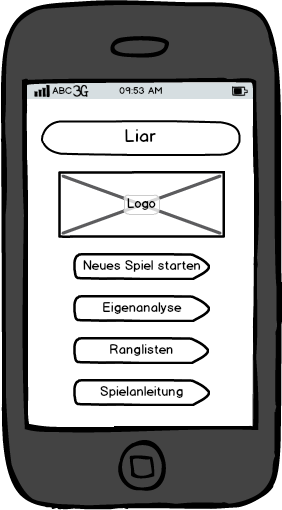
\includegraphics[width=0.3\textwidth]{mockup_01_index.png}
		\end{center}
		\caption[Mockup Hauptbildschirm]{Der Hauptbildschirms der LIAR-App umfasst die Menüpunkte: neues Spiel starten, Eigenanalyse, Ranglisten sowie Spielanleitung. }
		\label{fig:mockup_01}
	\end{figure}	
	\begin{figure}[h!]
		\begin{center}
			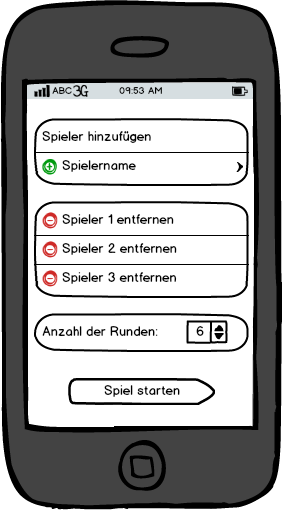
\includegraphics[width=0.3\textwidth]{mockup_02_newgame.png}
		\end{center}
		\caption[Mockup Bildschirm für neues Spiel]{Der Bildschirm für ein neues Spiel erlaubt das Festlegen der Spielernamen, der Spieleranzahl und der zu spielenden Runden.}
		\label{fig:mockup_02}
	\end{figure}	

	\newpage
	\begin{figure}[ht!]
		\begin{center}
			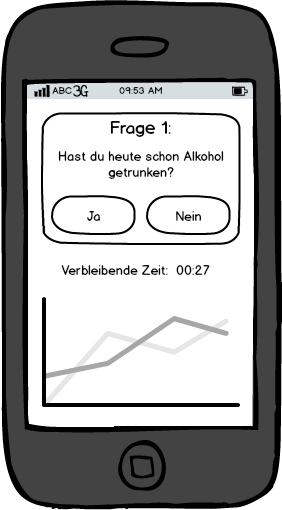
\includegraphics[width=0.3\textwidth]{mockup_03_playgame.png}
		\end{center}
		\caption[Mockup Spielbildschirm]{Der Spielbildschirm zeigt eine Frage, deren Antwortmöglichkeiten, die verstrichene Zeit, sowie den grafischen Verlauf der Sensordaten.}
		\label{fig:mockup_03}
	\end{figure}	
	\begin{figure}[h!]
		\begin{center}
			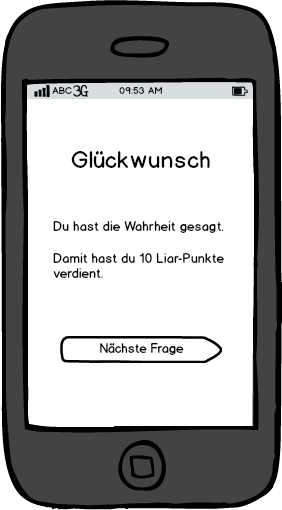
\includegraphics[width=0.3\textwidth]{mockup_04_score.png}
		\end{center}
		\caption[Mockup Bildschirm Fragenauswertung Wahrheit]{Auswertungsbildschirm bei wahrheitsgemäßer Antwort}
		\label{fig:mockup_04}
	\end{figure}	

	\newpage
	\begin{figure}[ht!]
		\begin{center}
			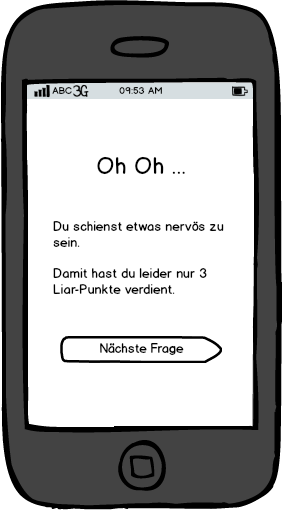
\includegraphics[width=0.3\textwidth]{mockup_05_score2.png}
		\end{center}
		\caption[Mockup Bildschirm Fragenauswertung Lüge]{Auswertungsbildschirm bei nicht wahrheitsgemäßer Antwort}
		\label{fig:mockup_05}
	\end{figure}	
	\begin{figure}[h!]
		\begin{center}
			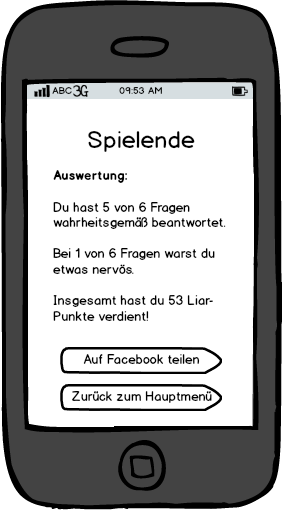
\includegraphics[width=0.3\textwidth]{mockup_06_finalscore.png}
		\end{center}
		\caption[Mockup finaler Bildschirm zur Fragenauswertung]{finaler Auswertungsbildschirm eines Spiels}
		\label{fig:mockup_06}
	\end{figure}	

	\newpage
	\begin{figure}[ht!]
		\begin{center}
			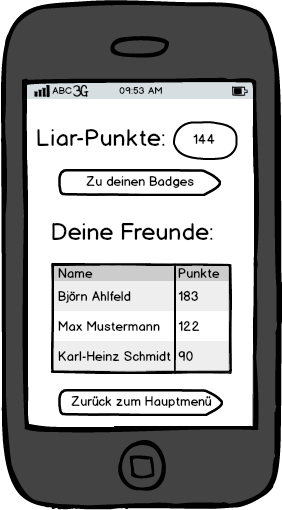
\includegraphics[width=0.3\textwidth]{mockup_07_ranking.png}
		\end{center}
		\caption[Mockup highscore-Bildschirm]{Der Ranking-Bildschirm zeigt die highscore-Einträge der Spieler}
		\label{fig:mockup_07}
	\end{figure}	
	\begin{figure}[h!]
		\begin{center}
			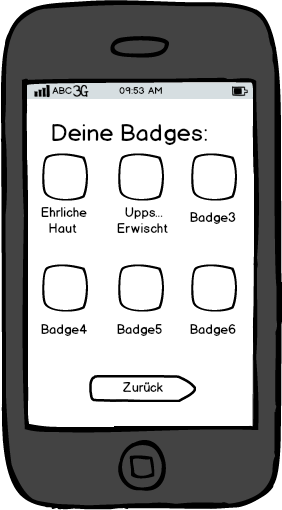
\includegraphics[width=0.3\textwidth]{mockup_08_badges.png}
		\end{center}
		\caption[Mockup Badge-Bildschirm]{Der Bildschirm zeigt das Badge-System, bei dem Spieler für bestimmte Leistungen Auszeichnungen erhalten.}
		\label{fig:mockup_08}
	\end{figure}	

	\newpage
	\begin{figure}[ht!]
		\begin{center}
			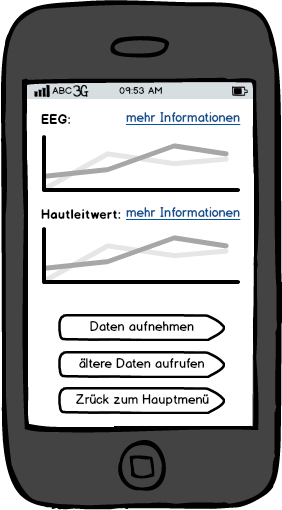
\includegraphics[width=0.3\textwidth]{mockup_09_selfanalysis.png}
		\end{center}
		\caption[Mockup Bildschirm Eigenanalyse]{Der Eigenanalyse-Bildschirm veranschaulicht die Messwerte aller Sensoren,erlaubt das Abspeichern von Daten, den Zugriff auf alte Daten und bietet Hilfetexte zu den verwendeten Sensoren an.}
		\label{fig:mockup_09}
	\end{figure}	
	\begin{figure}[h!]
		\begin{center}
			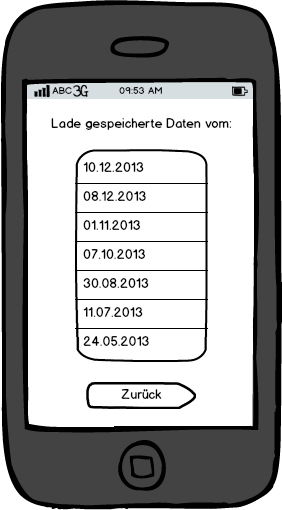
\includegraphics[width=0.3\textwidth]{mockup_10_saveddata.png}
		\end{center}
		\caption[Mockup Bildschirm zum Laden gespeicherter Daten]{Der Bildschirm zum Laden gespeicherter Daten erlaubt den Zugriff auf vergangene Eigenanalysen.}
		\label{fig:mockup_10}
	\end{figure}	
	
	\newpage
	\begin{figure}[ht!]
		\begin{center}
			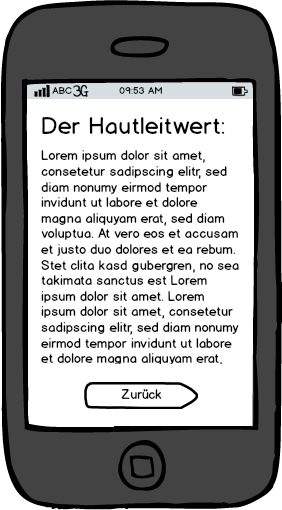
\includegraphics[width=0.3\textwidth]{mockup_11_skinconductance.png}
		\end{center}
		\caption[Mockup Infobildschirm Hautleitwert]{Der Informationsbildschirm Hautleitwert erklärt verständlich den genannten Sensor.}
		\label{fig:mockup_11}
	\end{figure}	
	\begin{figure}[h!]
		\begin{center}
			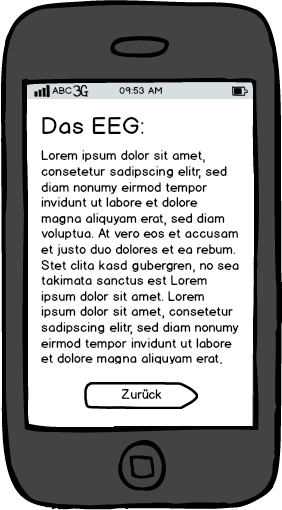
\includegraphics[width=0.3\textwidth]{mockup_12_eeg.png}
		\end{center}
		\caption[Mockup Infobildschirm EEG]{Der Informationsbildschirm EEG erklärt verständlich den genannten Sensor.}
		\label{fig:mockup_12}
	\end{figure}	

	\newpage
	\begin{figure}[ht!]
		\begin{center}
			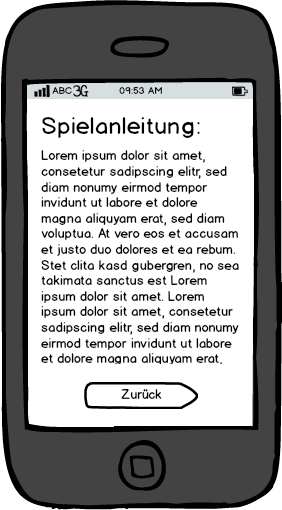
\includegraphics[width=0.3\textwidth]{mockup_13_instructions.png}
		\end{center}
		\caption[Mockup Anleitungsbildschirm]{Der Anleitungsbildschirm erklärt die wichtigsten Sachverhalte zu App und Sensoren.}
		\label{fig:mockup_13}
	\end{figure}	

   	%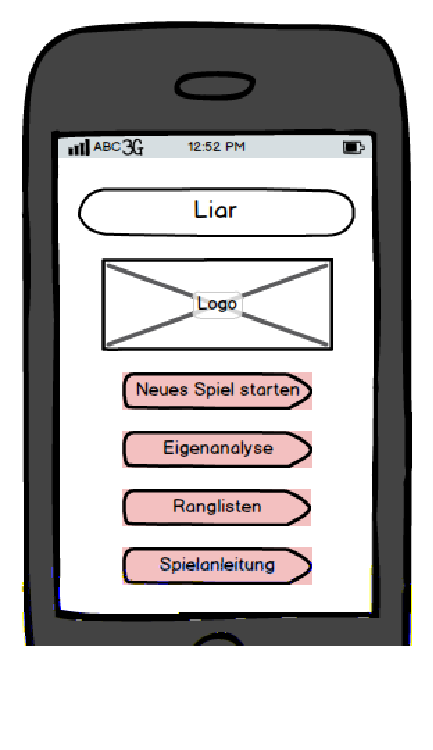
\includepdf[pagecommand={\thispagestyle{fancy}}, pages=1-13, scale=0.6, frame=true]{pdf/mockups.pdf}
